\documentclass[a4paper,11pt]{article}
\usepackage{amsmath,amssymb}
\usepackage[a4paper,left=19mm,right=19mm,top=40mm,bottom=40mm]{geometry}
\usepackage{txfonts}
\usepackage{kotex}
\usepackage{graphicx}
\usepackage{algorithm}
\usepackage{algpseudocode}
\usepackage{fancyvrb}

\begin{document}
\title{자료구조 HW11-HeapSort}
\author{B935394 컴퓨터공학과 장준희}
\maketitle
\newpage
\section{heap의 구현}
\ \ Max heap은 위에서부터 아래로, 왼쪽에서부터 오른쪽으로 채워나가기 때문에(완전 이진 트리 만족을 위해) 각 칸에 인덱스를 매겨줄 경우 배열로 힙을 구현하여도 공간의 낭비가 없다. 따라서 배열로 구현하기로 하였다. 다만 인덱스가 0부터 시작한다면 우리가 부모-자식 노드 관계를 표현할 때, $\times 2 /2$같은 연산을 이용하는데 있어 불편함이 있기 때문에, 1부터 시작하고 0은 공란으로 둔다.
\section{Adjust}
\ \ adjust함수는 부모노드와 자식 노드를 비교하며 최대 힙 구조가 될 때까지 아래(리프노드까지)로 내려가면서 비교하는 함수이다. 줄글로만 보았을 때는 이해가 전혀 가지않았기 때문에 이번 과제의 테스트케이스로 heapsort함수 안의 adjust함수가 어떻게 주어진 트리를 최대 힙 구조로 만드는지 살펴보려고 하였다. 그림으로 그리면 다음과 같다.
\begin{figure}[h]
\begin{center}
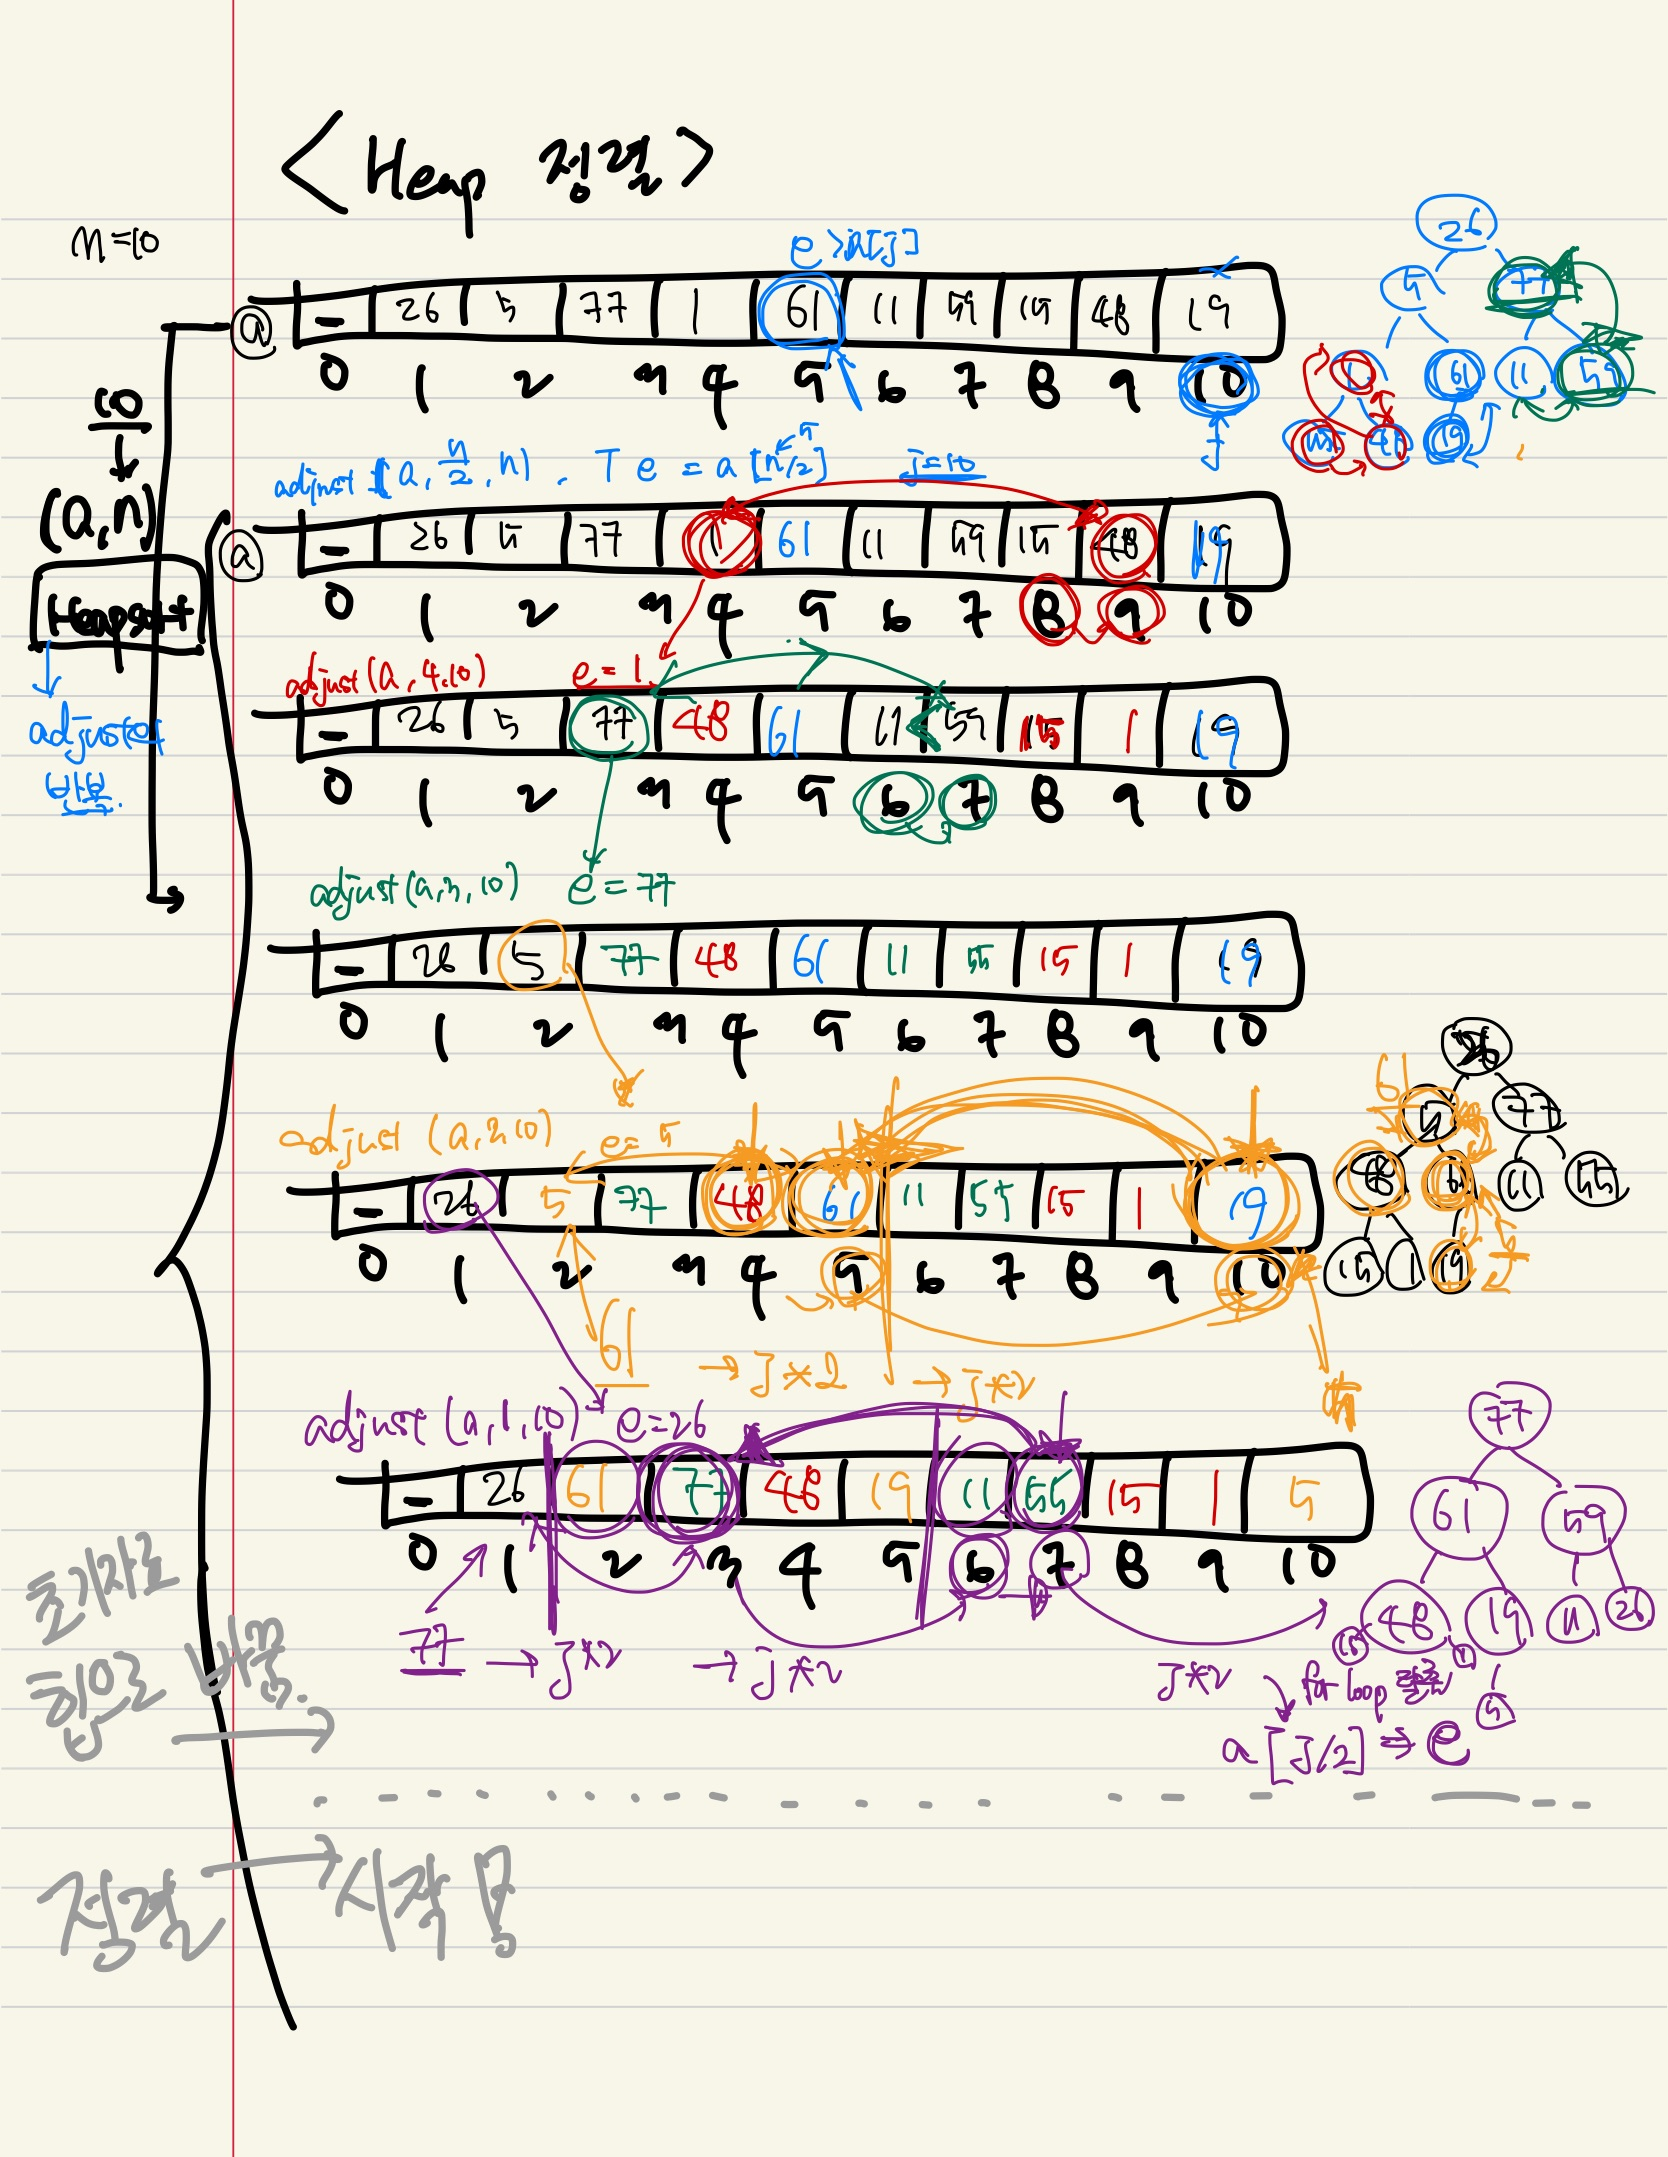
\includegraphics[width=0.6\textwidth]{heapsort}
\caption{Adjust}
\label{fig:fig1}
\end{center}
\end{figure}


노드의 수는 10개, 입력되는 수는 \{23,5,77,1,61,11,59,15,48,19\}이다.
다음은 heapsort함수 안에서 최대 힙으로 만드는 과정이다. (각 줄이 adjust함수가 하는 기능)
\begin{enumerate}
\item 가장 마지막부모([5])과 그 자식을 비교한 후, 부모가 더 크기 때문에 멈춘다.
\item 마지막에서 두번째 부모노드와 그 자식들을 비교한다. 작은 자식은 어차피 올라가면 최대 힙 구조를 만족하지 못하므로 자식들 중 큰 자식노드([9])와 부모노드([4])만 비교한다. 자식노드가 더 크기 때문에 자식노드의 값을 부모노드의 자리에 넣어둔다. 9*2를 하였더니 해당하는 인덱스가 없으므로 멈춘다.원래 부모노드의 값을 자식노드의 자리에 넣어준다.
\item 인덱스가 3이 된것과 자식노드간의 비교를 제외하면 동작은 1과 동일하다.
\item 초록색으로 표현된 노드들의 비교가 끝났음을 표현하기 위해 그려둔 것 같다.
\item \ [2]를 부모노드로 자식노드[4],[5]와 비교를 시작한다. [5]의 값이 더 크기 때문에 [2]와 [5]의 값을 비교한다. [5]의 값이 더 크므로 [5]의 값을 [2]에 넣는다. 현재[2]=61,[5]=61, [5*2]와 원래의 부모노드(5)와 비교를 한다. [10]의 값이 더 크므로 [10]의 값을 [5]에 넣어둔다. [10]의 자식은 없으므로 원래의 부모노드 값을 [10]에 넣는다.([2]=61,[5]=19,[10]=5)
\item \ [1]을 부모노드로 [2],[3]과 비교하고, 최대힙을 만족하지 않는다면 바꾸고, 다시 거기서 adjust를 해주고, 해준다.
\end{enumerate}
\ \ 이렇게 보고 나면 adjust함수는 위에서부터 시작해서 부모와 자식 노드를 비교해가며 자기가 영향을 끼친 subtree에 대해서는 부모 노드가 자식노드보다 크게끔 하는 것을 알 수 있다. 
\begin{Verbatim}
template <class T>
void HeapSort(T*a, const int n){
    for(int i=n/2;i>=1;i--){    //n/2는 가장 마지막 부모 노드
    //초기에 입력받은 인덱스들을 맥스힙으로 정렬해준다.
        adjust(a,i,n);
    }
    PrintArray(a,n);
    for(int i=n-1;i>=1;i--){        //한칸씩 줄여가며 정렬한다.
        swap(a[1],a[i+1]);         //현 히프의 처음과 마지막을 교환
        adjust(a,1,i);      //교환하면서, 망가진 힙구조를 되돌린다.
        PrintArray(a,i);
    }
}
\end{Verbatim} 
\ \ sort함수에서는 첫 for문에서 모든 부모노드들에 대해 adjust를 실행하고(MaxHeap으로 바꾸는 과정), 그 다음 for문에서는 루트 노드와 맨 마지막 노드 위치를 바꾸고 루트노드에 대해 adjust를 실행하여 최대힙 구조로 만들기를 반복하며 자료를 오름차순으로 정렬시키는 것을 알 수 있다.

\end{document}